\documentclass{standalone}
\usepackage{soul}
\usepackage{tikz}
\usetikzlibrary{circuits.logic.US,circuits.logic.IEC,shapes.geometric}
\usepackage{circuitikz}
\usepackage{adjustbox}

\begin{document}
\resizebox{\hsize}{!}{
\hspace{-4cm}
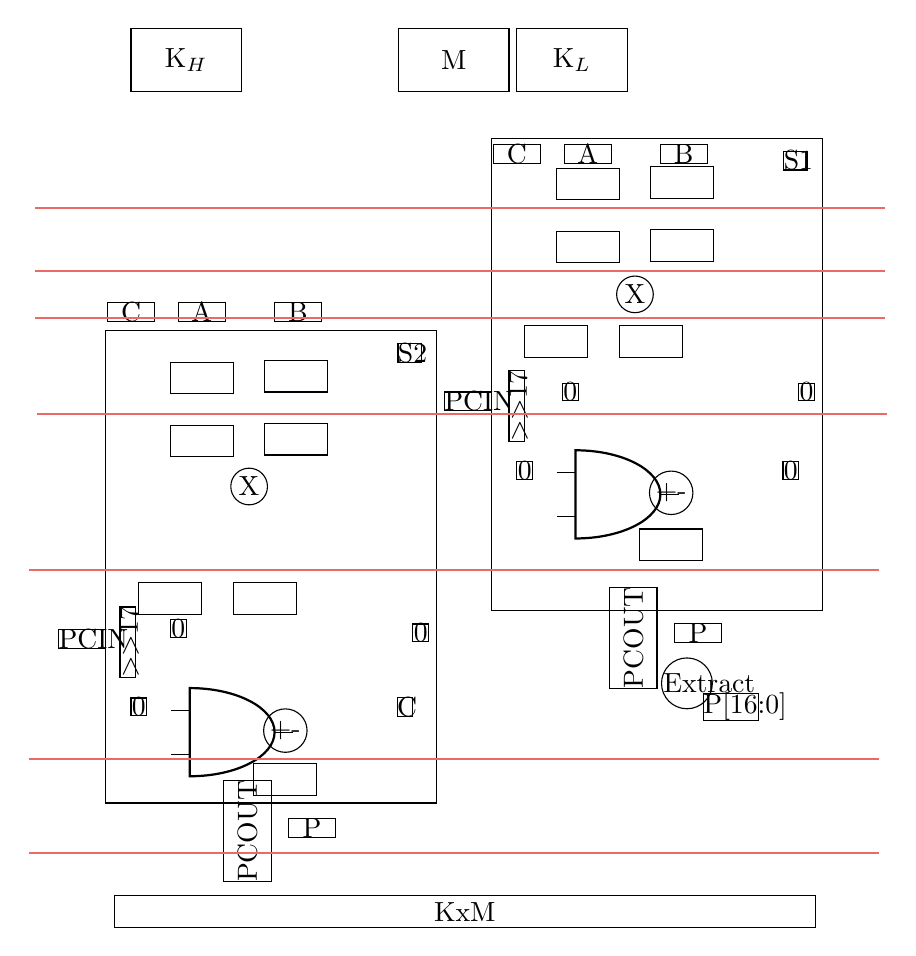
\begin{tikzpicture}[scale = 0.20]
\definecolor{FFFFFF}{RGB}{255,255,255}
\definecolor{009900}{RGB}{0,153,0}
\definecolor{EA6B66}{RGB}{234,107,102}
\definecolor{ffe6cc}{RGB}{255,230,204}
\definecolor{0000FF}{RGB}{0,0,255}
\node at (145.5,-47.6) [draw,solid,minimum width=4.2 cm,minimum height=6.0 cm,inner sep=0](ID2){};
\node at (144.1, -42.5)[circle,solid,minimum width=0.4 cm,minimum height=0.4 cm,text width=0.4cm,align=center,draw,inner sep=0](ID7){X};
\begin{scope}[shift={(145.2,-53.9)}]
\node at (1.2, -1.2)[circle,solid,minimum width=0.5 cm,minimum height=0.5 cm,text width=0.5cm,align=center,draw,inner sep=0](ID9){+-};
\node at (0.9,-1.3)[and port](ID10){};
\end{scope}
\node at (136.6, -49.6) [align=center,solid,draw,minimum width=0.2 cm,minimum height=0.5 cm,text width=0.2cm,inner sep=0](ID17) {\rotatebox{90}{$>$$>$17}};
\node at (155.0, -48.7) [align=center,solid,draw,minimum width=0.2 cm,minimum height=0.2 cm,text width=0.2cm,inner sep=0](ID18) {0};
\node at (140.0, -48.7) [align=center,solid,draw,minimum width=0.2 cm,minimum height=0.2 cm,text width=0.2cm,inner sep=0](ID19) {0};
\node at (133.5, -49.3) [align=center,solid,draw,minimum width=0.6 cm,minimum height=0.2 cm,text width=0.6cm,inner sep=0](ID20) {PCIN};
\node at (148.1, -64.0) [align=center,solid,draw,minimum width=0.6 cm,minimum height=0.2 cm,text width=0.6cm,inner sep=0](ID21) {P};
\node at (144.0, -64.3) [align=center,solid,draw,minimum width=0.6 cm,minimum height=0.2 cm,text width=0.6cm,inner sep=0](ID22) {\rotatebox{90}{PCOUT}};
\begin{scope}[shift={(145.1,-34.4)}]
\node at (2.0,-1.0) [draw,solid,minimum width=0.8 cm,minimum height=0.4 cm,inner sep=0](ID24){};
\end{scope}
\begin{scope}[shift={(145.1,-38.4)}]
\node at (2.0,-1.0) [draw,solid,minimum width=0.8 cm,minimum height=0.4 cm,inner sep=0](ID27){};
\end{scope}
\begin{scope}[shift={(139.1,-38.5)}]
\node at (2.0,-1.0) [draw,solid,minimum width=0.8 cm,minimum height=0.4 cm,inner sep=0](ID30){};
\end{scope}
\begin{scope}[shift={(139.1,-34.5)}]
\node at (2.0,-1.0) [draw,solid,minimum width=0.8 cm,minimum height=0.4 cm,inner sep=0](ID34){};
\end{scope}
\begin{scope}[shift={(137.1,-44.5)}]
\node at (2.0,-1.0) [draw,solid,minimum width=0.8 cm,minimum height=0.4 cm,inner sep=0](ID42){};
\end{scope}
\begin{scope}[shift={(143.1,-44.5)}]
\node at (2.0,-1.0) [draw,solid,minimum width=0.8 cm,minimum height=0.4 cm,inner sep=0](ID45){};
\end{scope}
\begin{scope}[shift={(144.4,-57.4)}]
\node at (2.0,-1.0) [draw,solid,minimum width=0.8 cm,minimum height=0.4 cm,inner sep=0](ID55){};
\end{scope}
\node at (154.3, -34.0) [align=center,solid,draw,minimum width=0.3 cm,minimum height=0.2 cm,text width=0.3cm,inner sep=0](ID63) {S1};
\node at (147.2, -33.6) [align=center,solid,draw,minimum width=0.6 cm,minimum height=0.2 cm,text width=0.6cm,inner sep=0](ID64) {B};
\node at (141.1, -33.6) [align=center,solid,draw,minimum width=0.6 cm,minimum height=0.2 cm,text width=0.6cm,inner sep=0](ID65) {A};
\node at (136.6, -33.6) [align=center,solid,draw,minimum width=0.6 cm,minimum height=0.2 cm,text width=0.6cm,inner sep=0](ID66) {C};
\node at (147.4, -67.2)[circle,solid,minimum width=0.6 cm,minimum height=0.6 cm,text width=0.6cm,align=center,draw,inner sep=0](ID72){Extract};
\node at (150.2, -68.7) [align=center,solid,draw,minimum width=0.7 cm,minimum height=0.2 cm,text width=0.7cm,inner sep=0](ID75) {P[16:0]};
\node at (133.3, -81.7) [align=center,solid,draw,minimum width=8.9 cm,minimum height=0.4 cm,text width=8.9cm,inner sep=0](ID76) {KxM};
\node at (121.0,-59.8) [draw,solid,minimum width=4.2 cm,minimum height=6.0 cm,inner sep=0](ID79){};
\node at (119.6, -54.7)[circle,solid,minimum width=0.4 cm,minimum height=0.4 cm,text width=0.4cm,align=center,draw,inner sep=0](ID84){X};
\begin{scope}[shift={(120.7,-69.0)}]
\node at (1.2, -1.2)[circle,solid,minimum width=0.5 cm,minimum height=0.5 cm,text width=0.5cm,align=center,draw,inner sep=0](ID86){+-};
\node at (0.9,-1.3)[and port](ID87){};
\end{scope}
\node at (111.9, -64.6) [align=center,solid,draw,minimum width=0.2 cm,minimum height=0.5 cm,text width=0.2cm,inner sep=0](ID93) {\rotatebox{90}{$>$$>$17}};
\node at (130.5, -64.0) [align=center,solid,draw,minimum width=0.2 cm,minimum height=0.2 cm,text width=0.2cm,inner sep=0](ID94) {0};
\node at (115.1, -63.7) [align=center,solid,draw,minimum width=0.2 cm,minimum height=0.2 cm,text width=0.2cm,inner sep=0](ID95) {0};
\node at (109.0, -64.4) [align=center,solid,draw,minimum width=0.6 cm,minimum height=0.2 cm,text width=0.6cm,inner sep=0](ID96) {PCIN};
\node at (123.6, -76.4) [align=center,solid,draw,minimum width=0.6 cm,minimum height=0.2 cm,text width=0.6cm,inner sep=0](ID97) {P};
\node at (119.5, -76.6) [align=center,solid,draw,minimum width=0.6 cm,minimum height=0.2 cm,text width=0.6cm,inner sep=0](ID98) {\rotatebox{90}{PCOUT}};
\begin{scope}[shift={(120.6,-46.7)}]
\node at (2.0,-1.0) [draw,solid,minimum width=0.8 cm,minimum height=0.4 cm,inner sep=0](ID100){};
\end{scope}
\begin{scope}[shift={(120.6,-50.7)}]
\node at (2.0,-1.0) [draw,solid,minimum width=0.8 cm,minimum height=0.4 cm,inner sep=0](ID103){};
\end{scope}
\begin{scope}[shift={(114.6,-50.8)}]
\node at (2.0,-1.0) [draw,solid,minimum width=0.8 cm,minimum height=0.4 cm,inner sep=0](ID106){};
\end{scope}
\begin{scope}[shift={(114.6,-46.8)}]
\node at (2.0,-1.0) [draw,solid,minimum width=0.8 cm,minimum height=0.4 cm,inner sep=0](ID109){};
\end{scope}
\begin{scope}[shift={(112.6,-60.8)}]
\node at (2.0,-1.0) [draw,solid,minimum width=0.8 cm,minimum height=0.4 cm,inner sep=0](ID112){};
\end{scope}
\begin{scope}[shift={(118.6,-60.8)}]
\node at (2.0,-1.0) [draw,solid,minimum width=0.8 cm,minimum height=0.4 cm,inner sep=0](ID115){};
\end{scope}
\begin{scope}[shift={(119.9,-72.3)}]
\node at (2.0,-1.0) [draw,solid,minimum width=0.8 cm,minimum height=0.4 cm,inner sep=0](ID125){};
\end{scope}
\node at (129.8, -46.2) [align=center,solid,draw,minimum width=0.3 cm,minimum height=0.2 cm,text width=0.3cm,inner sep=0](ID132) {S2};
\node at (122.7, -43.6) [align=center,solid,draw,minimum width=0.6 cm,minimum height=0.2 cm,text width=0.6cm,inner sep=0](ID133) {B};
\node at (116.6, -43.6) [align=center,solid,draw,minimum width=0.6 cm,minimum height=0.2 cm,text width=0.6cm,inner sep=0](ID134) {A};
\node at (112.1, -43.6) [align=center,solid,draw,minimum width=0.6 cm,minimum height=0.2 cm,text width=0.6cm,inner sep=0](ID135) {C};
\node at (132.6, -27.6) [align=center,solid,draw,minimum width=1.4 cm,minimum height=0.8 cm,text width=1.4cm,inner sep=0](ID136) {M};
\node at (140.1, -27.6) [align=center,solid,draw,minimum width=1.4 cm,minimum height=0.8 cm,text width=1.4cm,inner sep=0](ID137) {K$_L$};
\node at (115.6, -27.6) [align=center,solid,draw,minimum width=1.4 cm,minimum height=0.8 cm,text width=1.4cm,inner sep=0](ID138) {K$_H$};
\node at (154.0, -53.7) [align=center,solid,draw,minimum width=0.2 cm,minimum height=0.2 cm,text width=0.2cm,inner sep=0](ID143) {0};
\node at (137.1, -53.7) [align=center,solid,draw,minimum width=0.2 cm,minimum height=0.2 cm,text width=0.2cm,inner sep=0](ID144) {0};
\node at (129.5, -68.7) [align=center,solid,draw,minimum width=0.2 cm,minimum height=0.2 cm,text width=0.2cm,inner sep=0](ID145) {C};
\node at (112.6, -68.7) [align=center,solid,draw,minimum width=0.2 cm,minimum height=0.2 cm,text width=0.2cm,inner sep=0](ID150) {0};
\draw [solid,EA6B66,line width=0.7pt] (106.0,-44.0)--(160.0,-44.0);
\draw [solid,EA6B66,line width=0.7pt] (106.1,-50.1)--(160.1,-50.1);
\draw [solid,EA6B66,line width=0.7pt] (105.6,-60.0)--(159.6,-60.0);
\draw [solid,EA6B66,line width=0.7pt] (105.6,-78.0)--(159.6,-78.0);
\draw [solid,EA6B66,line width=0.7pt] (106.0,-37.0)--(160.0,-37.0);
\draw [solid,EA6B66,line width=0.7pt] (106.0,-41.0)--(160.0,-41.0);
\draw [solid,EA6B66,line width=0.7pt] (105.6,-72.0)--(159.6,-72.0);
\end{tikzpicture}
}
\end{document}
